\documentclass[tikz,border=8pt]{standalone}
% Shared pastel academic grammar for final-size technical-paper diagrams.
\usepackage[T1]{fontenc}
\usepackage{lmodern}
\usepackage{amsmath,amssymb}
\usepackage{xcolor}
\usepackage{tikz}
\usetikzlibrary{
  arrows.meta,
  backgrounds,
  calc,
  circuits.logic.US,
  decorations.pathreplacing,
  fit,
  matrix,
  patterns,
  positioning,
  shapes.geometric,
  shapes.symbols
}

\definecolor{ink}{RGB}{24,24,28}
\definecolor{midink}{RGB}{96,96,104}
\definecolor{paleink}{RGB}{184,184,190}
\definecolor{wash}{RGB}{241,240,237}
\definecolor{paper}{RGB}{255,255,253}
\definecolor{cyan}{RGB}{126,203,218}
\definecolor{cyanwash}{RGB}{211,238,242}
\definecolor{pink}{RGB}{235,139,158}
\definecolor{pinkwash}{RGB}{250,211,217}
\definecolor{purple}{RGB}{166,50,150}
\definecolor{purplewash}{RGB}{232,196,227}
\definecolor{gold}{RGB}{177,139,45}
\definecolor{goldwash}{RGB}{239,226,183}
\definecolor{slate}{RGB}{116,133,145}
\definecolor{slatewash}{RGB}{221,226,229}
\colorlet{muted}{midink}
\colorlet{rule}{paleink}
\colorlet{accent}{purple}
\colorlet{accentwash}{purplewash}
\colorlet{second}{cyan}
\colorlet{secondwash}{cyanwash}

\tikzset{
  every picture/.style={
    font=\rmfamily\footnotesize,
    text=ink,
    line cap=round,
    line join=round,
    >=Stealth
  },
  every node/.style={outer sep=0pt},
  panel mark/.style={font=\rmfamily\bfseries\footnotesize},
  primary/.style={font=\rmfamily\footnotesize},
  secondary/.style={font=\rmfamily\scriptsize,text=midink},
  signal name/.style={font=\ttfamily\footnotesize,anchor=east},
  scope trace/.style={draw=ink,line width=.62pt,line cap=butt,line join=miter},
  hairline/.style={draw=paleink,line width=.28pt,line cap=butt},
  dotted guide/.style={draw=midink,line width=.32pt,densely dotted},
  dashed scope/.style={draw=ink,line width=.45pt,dashed},
  transition/.style={-{Stealth[length=1.8mm,width=1.25mm]},draw=ink,line width=.58pt},
  transition label/.style={font=\rmfamily\scriptsize,fill=paper,inner sep=1.2pt},
  preedge/.style={circle,draw=ink,fill=paper,line width=.58pt,minimum size=8.2mm,inner sep=1pt},
  observed preedge/.style={preedge,fill=purplewash,double,double distance=1.15pt,line width=.62pt,minimum size=9.8mm},
  brace/.style={decorate,decoration={brace,mirror,amplitude=3pt},draw=ink,line width=.45pt},
  grid rule/.style={draw=slate,line width=.32pt,line cap=butt},
  outer rule/.style={draw=ink,line width=.82pt,line cap=butt,line join=miter},
  star mark/.style={star,star points=5,star point ratio=2.2,draw=ink,fill=purple,minimum size=5.1mm,inner sep=0pt},
  % Compatibility vocabulary used by the repository's other figures.
  flow/.style={-{Latex[length=4.5pt,width=3.2pt]},draw=ink,line width=.55pt},
  heavy flow/.style={-{Latex[length=5pt,width=3.6pt]},draw=ink,line width=.8pt},
  wire/.style={draw=ink,line width=.5pt},
  bus/.style={draw=ink,line width=1.05pt},
  guide/.style={draw=midink,line width=.4pt,dotted},
  alternate/.style={draw=ink,line width=.5pt,dashed},
  scope/.style={draw=ink,line width=.5pt,dashed,inner sep=6pt},
  block/.style={draw=ink,line width=.55pt,fill=paper,minimum height=8mm,inner xsep=5pt,inner ysep=4pt,align=center},
  operation/.style={block,fill=cyanwash,minimum width=17mm},
  register/.style={block,fill=paper,minimum width=16mm,minimum height=10mm},
  state/.style={circle,draw=ink,line width=.55pt,fill=cyanwash,minimum size=8mm,inner sep=1pt,align=center},
  terminal/.style={state,fill=purplewash,double,double distance=1.2pt,line width=.6pt},
  predicate/.style={diamond,aspect=1.8,draw=ink,line width=.55pt,fill=pinkwash,inner xsep=3pt,inner ysep=2pt,align=center},
  datum/.style={rectangle,draw=ink,line width=.5pt,fill=goldwash,minimum width=8mm,minimum height=6mm,inner sep=2pt,align=center},
  panel label/.style={font=\rmfamily\bfseries\footnotesize},
  local heading/.style={font=\rmfamily\bfseries\footnotesize},
  annotation/.style={font=\rmfamily\scriptsize,text=midink,align=center},
  heading/.style={font=\rmfamily\bfseries\small},
  subheading/.style={font=\rmfamily\bfseries\footnotesize},
  note/.style={font=\rmfamily\scriptsize,text=midink},
  label/.style={font=\rmfamily\bfseries\scriptsize},
  mono/.style={font=\ttfamily\footnotesize},
  tiny mono/.style={font=\ttfamily\scriptsize},
  count/.style={font=\rmfamily\bfseries\small},
  selected/.style={draw=ink,fill=purplewash,line width=.8pt},
  cell on/.style={fill=purple,draw=ink,line width=.3pt},
  cell off/.style={fill=paper,draw=paleink,line width=.3pt}
}

% Flat pastel facets and depth edges for restrained axonometric constructions.
\tikzset{
  cyan facet/.style={draw=ink,fill=cyanwash,line width=.5pt,line join=round},
  cyan side/.style={draw=ink,fill=cyan,line width=.5pt,line join=round},
  pink facet/.style={draw=ink,fill=pinkwash,line width=.5pt,line join=round},
  pink side/.style={draw=ink,fill=pink,line width=.5pt,line join=round},
  purple facet/.style={draw=ink,fill=purplewash,line width=.55pt,line join=round},
  purple side/.style={draw=ink,fill=purple,line width=.55pt,line join=round},
  gold facet/.style={draw=ink,fill=goldwash,line width=.5pt,line join=round},
  gold side/.style={draw=ink,fill=gold,line width=.5pt,line join=round},
  context facet/.style={draw=ink,fill=slatewash,line width=.45pt,line join=round},
  depth edge/.style={draw=midink,line width=.38pt},
  surface grid/.style={draw=slate,line width=.32pt},
  projection/.style={draw=midink,line width=.38pt,densely dashed},
  accent curve/.style={draw=purple,line width=1.05pt},
  cyan curve/.style={draw=cyan!70!ink,line width=.9pt},
  pink curve/.style={draw=pink!70!ink,line width=.9pt},
  gold curve/.style={draw=gold!80!ink,line width=.9pt}
}

\usetikzlibrary{circuits.logic.US}

\tikzset{
  local heading/.style={font=\rmfamily\bfseries\footnotesize},
  annotation/.style={secondary,align=center},
  mono/.style={font=\ttfamily\footnotesize},
  wire/.style={scope trace,line width=.5pt},
  guide/.style={dotted guide},
  flow/.style={transition},
  heavy flow/.style={transition,line width=.82pt},
  rule/.style={hairline},
  route contact/.style={
    circle,draw=ink,line width=.5pt,minimum size=3.0mm,inner sep=0pt
  },
  model port/.style={
    circle,draw=ink,fill=paper,line width=.5pt,minimum size=2.5mm,inner sep=0pt
  },
  gate symbol/.style={
    draw=ink,line width=.6pt,minimum width=11.5mm,minimum height=8.5mm
  },
  vector text/.style={font=\ttfamily\scriptsize,anchor=west}
}

\begin{document}
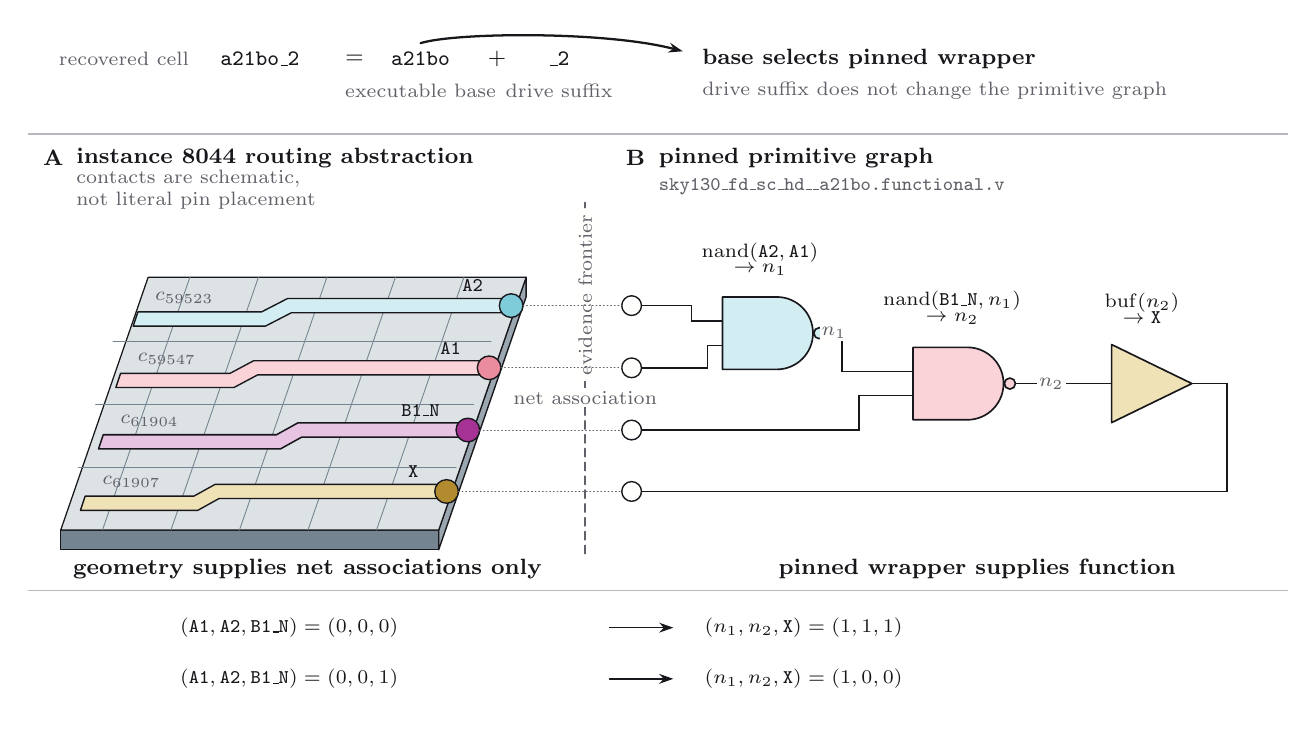
\begin{tikzpicture}[x=1cm,y=1cm]
  \path[use as bounding box] (0,0) rectangle (16,8.7);

  % Qualified layout name: only the base chooses executable behavior.
  \node[annotation,anchor=west] at (.28,8.30) {recovered cell};
  \node[mono] (qualified) at (2.95,8.30) {\texttt{a21bo\_2}};
  \node at (4.15,8.30) {$=$};
  \node[mono] (base) at (4.99,8.30) {\texttt{a21bo}};
  \node at (5.96,8.30) {$+$};
  \node[mono] (suffix) at (6.75,8.30) {\texttt{\_2}};
  \node[annotation] at (4.99,7.90) {executable base};
  \node[annotation] at (6.75,7.90) {drive suffix};
  \draw[heavy flow]
    (base.north) .. controls (5.42,8.64) and (7.34,8.66) .. (8.32,8.40);
  \node[local heading,anchor=west] at (8.45,8.30)
    {base selects pinned wrapper};
  \node[annotation,anchor=west] at (8.45,7.90)
    {drive suffix does not change the primitive graph};
  \draw[rule,line width=.45pt] (0,7.35) -- (16,7.35);

  % Left: an axonometric abstraction of routing-derived net association.
  \node[panel mark,anchor=west] at (.08,7.04) {A};
  \node[local heading,anchor=west] at (.50,7.04)
    {instance 8044 routing abstraction};
  \node[annotation,anchor=west,align=left] at (.50,6.64)
    {contacts are schematic,\\not literal pin placement};

  % The slab has shallow depth, a sparse surface grid, and four net ribbons.
  \path[fill=slate,draw=ink,line width=.5pt]
    (.42,2.32) -- (5.22,2.32) -- (5.22,2.07) -- (.42,2.07) -- cycle;
  \path[fill=slate!72,draw=ink,line width=.5pt]
    (5.22,2.32) -- (6.33,5.53) -- (6.33,5.28) -- (5.22,2.07) -- cycle;
  \path[context facet]
    (.42,2.32) -- (5.22,2.32) -- (6.33,5.53) -- (1.53,5.53) -- cycle;
  \foreach \x in {.95,1.82,2.69,3.56,4.43}{
    \draw[surface grid] (\x,2.32) -- ($ (\x,2.32)+(1.11,3.21) $);
  }
  \foreach \d in {.80,1.60,2.40}{
    \draw[surface grid]
      ($(.42,2.32)+(0.277*\d,\d)$) --
      ($(5.22,2.32)+(0.277*\d,\d)$);
  }

  % A2 / c59523, cyan ribbon.
  \path[cyan facet]
    (1.34,4.91) -- (3.02,4.91) -- (3.35,5.08) -- (6.08,5.08) --
    (6.15,5.26) -- (3.30,5.26) -- (2.97,5.09) -- (1.40,5.09) -- cycle;
  \node[route contact,fill=cyan] (ra2) at (6.14,5.17) {};
  \node[annotation,anchor=west] at (1.50,5.27) {$c_{59523}$};
  \node[font=\ttfamily\scriptsize,anchor=east] at (5.90,5.42) {A2};

  % A1 / c59547, coral ribbon.
  \path[pink facet]
    (1.12,4.13) -- (2.62,4.13) -- (2.92,4.29) -- (5.80,4.29) --
    (5.87,4.47) -- (2.87,4.47) -- (2.57,4.31) -- (1.18,4.31) -- cycle;
  \node[route contact,fill=pink] (ra1) at (5.86,4.38) {};
  \node[annotation,anchor=west] at (1.28,4.49) {$c_{59547}$};
  \node[font=\ttfamily\scriptsize,anchor=east] at (5.62,4.63) {A1};

  % B1_N / c61904, magenta ribbon.
  \path[purple facet]
    (.90,3.35) -- (3.21,3.35) -- (3.48,3.50) -- (5.53,3.50) --
    (5.60,3.68) -- (3.43,3.68) -- (3.16,3.53) -- (.96,3.53) -- cycle;
  \node[route contact,fill=purple] (rb1) at (5.59,3.59) {};
  \node[annotation,anchor=west] at (1.06,3.71) {$c_{61904}$};
  \node[font=\ttfamily\scriptsize,anchor=east] at (5.35,3.84) {B1\_N};

  % X / c61907, ochre ribbon.
  \path[gold facet]
    (.67,2.57) -- (2.16,2.57) -- (2.43,2.72) -- (5.26,2.72) --
    (5.33,2.90) -- (2.38,2.90) -- (2.11,2.75) -- (.73,2.75) -- cycle;
  \node[route contact,fill=gold] (rx) at (5.32,2.81) {};
  \node[annotation,anchor=west] at (.83,2.93) {$c_{61907}$};
  \node[font=\ttfamily\scriptsize,anchor=east] at (5.08,3.06) {X};

  \node[local heading,anchor=west] at (.46,1.82)
    {geometry supplies net associations only};

  % The frontier separates geometric association from executable semantics.
  \draw[projection,line width=.55pt] (7.08,2.02) -- (7.08,6.48);
  \node[annotation,rotate=90,fill=paper,inner sep=2pt] at (7.08,5.30)
    {evidence frontier};
  \node[model port] (ma2) at (7.67,5.17) {};
  \node[model port] (ma1) at (7.67,4.38) {};
  \node[model port] (mb1) at (7.67,3.59) {};
  \node[model port] (mx) at (7.67,2.81) {};
  \draw[guide] (ra2) -- (ma2);
  \draw[guide] (ra1) -- (ma1);
  \draw[guide] (rb1) -- (mb1);
  \draw[guide] (rx) -- (mx);
  \node[annotation,fill=paper,inner sep=1pt] at (7.08,4.00)
    {net association};

  % Right: exact two-NAND-and-buffer graph from the pinned raw wrapper.
  \node[panel mark,anchor=west] at (7.48,7.04) {B};
  \node[local heading,anchor=west] at (7.90,7.04)
    {pinned primitive graph};
  \node[annotation,anchor=west] at (7.90,6.68)
    {\texttt{sky130\_fd\_sc\_hd\_\_a21bo.functional.v}};

  \node[nand gate US,gate symbol,fill=cyanwash,logic gate inputs=nn] (nand0)
    at (9.36,4.82) {};
  \node[nand gate US,gate symbol,fill=pinkwash,logic gate inputs=nn] (nand1)
    at (11.78,4.18) {};
  \node[buffer gate US,gate symbol,fill=goldwash] (buf0) at (14.12,4.18) {};

  \draw[wire] (ma2) -- (8.43,5.17) |- (nand0.input 1);
  \draw[wire] (ma1) -- (8.63,4.38) |- (nand0.input 2);
  \draw[wire] (nand0.output) -- (10.34,4.82) |- (nand1.input 1);
  \node[annotation,fill=paper,inner sep=.8pt] at (10.24,4.82) {$n_1$};
  \draw[wire] (mb1) -- (10.56,3.59) |- (nand1.input 2);
  \draw[wire] (nand1.output) -- (buf0.input);
  \node[annotation,fill=paper,inner sep=.8pt] at (13.00,4.18) {$n_2$};
  \draw[wire] (buf0.output) -- (15.23,4.18) -- (15.23,2.81) -- (mx);

  \node[font=\ttfamily\scriptsize,align=center] at (9.30,5.76)
    {$\operatorname{nand}(\texttt{A2},\texttt{A1})$\\[-.8mm]$\to n_1$};
  \node[font=\ttfamily\scriptsize,align=center] at (11.74,5.14)
    {$\operatorname{nand}(\texttt{B1\_N},n_1)$\\[-.8mm]$\to n_2$};
  \node[font=\ttfamily\scriptsize,align=center] at (14.15,5.14)
    {$\operatorname{buf}(n_2)$\\[-.8mm]$\to\texttt{X}$};

  \node[local heading,anchor=west] at (9.42,1.82)
    {pinned wrapper supplies function};

  % Two exact executions of the serialized raw wrapper.
  \draw[rule,line width=.45pt] (0,1.55) -- (16,1.55);
  \node[vector text] at (1.82,1.08)
    {$(\texttt{A1},\texttt{A2},\texttt{B1\_N})=(0,0,0)$};
  \draw[flow] (7.39,1.08) -- (8.20,1.08);
  \node[vector text] at (8.48,1.08)
    {$(n_1,n_2,\texttt{X})=(1,1,1)$};

  \node[vector text] at (1.82,.43)
    {$(\texttt{A1},\texttt{A2},\texttt{B1\_N})=(0,0,1)$};
  \draw[flow] (7.39,.43) -- (8.20,.43);
  \node[vector text] at (8.48,.43)
    {$(n_1,n_2,\texttt{X})=(1,0,0)$};
\end{tikzpicture}
\end{document}
